% 图 22.5 —— 由 `checks/emit_hand.py` 自动拼出（probe 精测 + prims2 图元分解）
%%
% ⚠ 这是**稿子不是成品**：跑 `checks/checkhand.py 22.5` 看指标 + 看叠合图。
%%
%% ⚠ 待核：
%   · 本图 probe 报出阴影族 1 个 —— **本脚本不生成阴影**（要照原书手写）；prims2 的 strokes 里可能含阴影线，核对时留意别画重
%   · 可疑字形 1 项（空心圈 ⊙ 常被认成字母 o）—— 见文件末
%%
\documentclass[12pt]{standalone}
\usepackage{fontspec}
\setsansfont{Arial}
\newfontfamily\mfallback{DejaVu Sans}
\usepackage{tikz}
\begin{document}
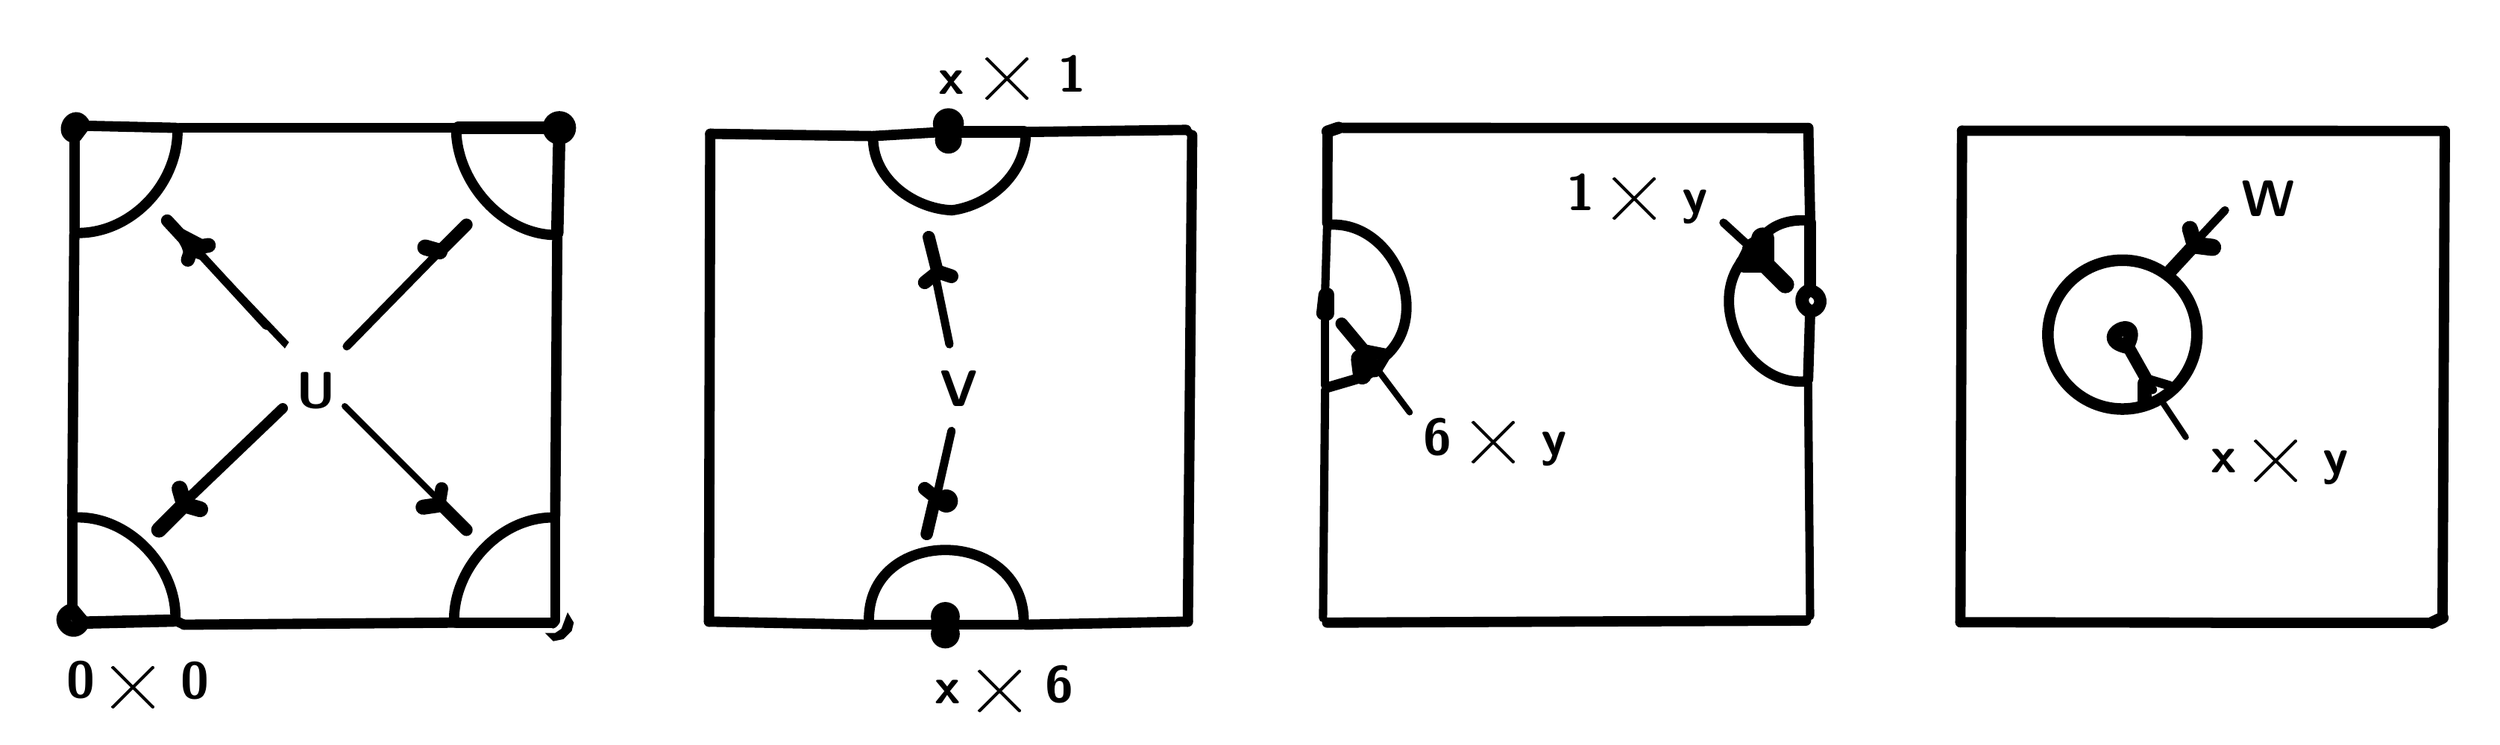
\begin{tikzpicture}[x=1pt, y=-1pt, line width=5.6pt, line cap=round, line join=round]

  %% ════ 填充区（prims2 的 fills）════
  \fill (71.0,97.0) -- (78.0,110.0) -- (81.0,119.0) -- (84.0,115.0) -- (87.0,116.0) -- (128.0,159.0) -- (130.0,156.0) -- (89.0,113.0) -- (92.0,108.0) -- cycle;
  \fill (265.0,287.0) -- (262.0,295.0) -- (259.0,297.0) -- (254.0,297.0) -- (258.0,301.0) -- (263.0,300.0) -- (267.0,296.0) -- (268.0,292.0) -- cycle;

  %% ════ 直线段（prims2 的 strokes）════
  \draw[line width=6.0pt] (486.0,54.0) -- (451.0,54.0);
  \draw[line width=6.5pt] (438.0,227.0) -- (443.0,231.0);
  \draw[line width=7.5pt] (79.0,235.0) -- (67.0,247.0);
  \draw[line width=3.0pt] (1049.0,202.0) -- (1037.0,184.0);
  \draw[line width=5.0pt] (650.0,173.0) -- (633.0,178.0);
  \draw[line width=6.0pt] (640.0,147.0) -- (650.0,159.0);
  \draw[line width=6.0pt] (651.0,172.0) -- (656.0,169.0);
  \draw[line width=6.0pt] (843.0,106.0) -- (838.0,109.0);
  \draw[line width=5.0pt] (412.0,56.0) -- (334.1,54.9);
  \draw[line width=5.0pt] (334.1,54.9) -- (333.5,291.5);
  \draw[line width=5.0pt] (333.5,291.5) -- (410.0,293.0);
  \draw[line width=7.7pt] (203.0,112.0) -- (196.0,110.0);
  \draw[line width=4.0pt] (202.0,113.0) -- (158.0,158.0);
  \draw[line width=5.0pt] (488.0,54.0) -- (564.7,53.0);
  \draw[line width=3.9pt] (564.7,53.0) -- (567.6,55.6);
  \draw[line width=5.0pt] (567.6,55.6) -- (565.5,291.5);
  \draw[line width=5.0pt] (565.5,291.5) -- (487.0,293.0);
  \draw[line width=3.0pt] (203.0,233.0) -- (157.0,187.0);
  \draw[line width=6.3pt] (203.0,233.0) -- (204.0,227.0);
  \draw[line width=7.7pt] (77.0,227.0) -- (79.0,234.0);
  \draw[line width=9.0pt] (649.0,164.0) -- (650.0,172.0);
  \draw[line width=5.0pt] (259.0,241.0) -- (259.0,291.0);
  \draw[line width=8.0pt] (651.0,163.0) -- (656.0,169.0);
  \draw[line width=8.7pt] (835.0,118.0) -- (843.0,118.0);
  \draw[line width=6.0pt] (661.0,162.0) -- (651.0,160.0);
  \draw[line width=5.0pt] (25.0,240.0) -- (26.0,104.0);
  \draw[line width=4.0pt] (85.0,111.0) -- (119.0,148.0);
  \draw[line width=6.0pt] (204.0,111.0) -- (216.0,99.0);
  \draw[line width=6.5pt] (438.0,127.0) -- (443.0,123.0);
  \draw[line width=6.7pt] (451.0,124.0) -- (445.0,122.0);
  \draw[line width=8.3pt] (1062.0,110.0) -- (1054.0,109.0);
  \draw[line width=7.7pt] (1053.0,108.0) -- (1051.0,101.0);
  \draw[line width=6.0pt] (867.0,130.0) -- (867.0,98.0);
  \draw[line width=5.0pt] (633.0,98.0) -- (633.2,53.8);
  \draw[line width=5.9pt] (633.2,53.8) -- (638.5,52.0);
  \draw[line width=5.0pt] (638.5,52.0) -- (866.1,52.1);
  \draw[line width=5.0pt] (866.1,52.1) -- (867.0,96.0);
  \draw[line width=5.0pt] (25.0,242.0) -- (25.0,286.0);
  \draw[line width=4.0pt] (443.0,123.0) -- (450.0,157.0);
  \draw[line width=7.3pt] (202.0,235.0) -- (195.0,236.0);
  \draw[line width=5.0pt] (658.0,168.0) -- (661.0,163.0);
  \draw[line width=6.0pt] (439.0,249.0) -- (443.0,232.0);
  \draw[line width=5.0pt] (127.0,188.0) -- (80.0,233.0);
  \draw[line width=4.0pt] (825.0,98.0) -- (837.0,109.0);
  \draw[line width=4.0pt] (444.0,230.0) -- (451.0,199.0);
  \draw[line width=5.0pt] (866.0,174.0) -- (867.0,142.0);
  \draw[line width=6.0pt] (440.0,105.0) -- (444.0,121.0);
  \draw[line width=5.0pt] (257.0,292.0) -- (211.0,292.0);
  \draw[line width=3.0pt] (658.0,170.0) -- (673.0,190.0);
  \draw[line width=4.0pt] (1068.0,92.0) -- (1054.0,107.0);
  \draw[line width=4.0pt] (866.0,176.0) -- (867.0,288.8);
  \draw[line width=2.9pt] (867.0,288.8) -- (865.0,291.0);
  \draw[line width=5.0pt] (865.0,291.0) -- (633.0,292.0);
  \draw[line width=2.9pt] (633.0,292.0) -- (631.0,289.8);
  \draw[line width=4.0pt] (631.0,289.8) -- (632.0,179.0);
  \draw[line width=6.0pt] (204.0,235.0) -- (216.0,247.0);
  \draw[line width=6.5pt] (632.0,133.0) -- (631.0,142.0);
  \draw[line width=3.7pt] (259.0,292.0) -- (258.0,293.0);
  \draw[line width=7.0pt] (30.0,292.0) -- (25.0,286.0);
  \draw[line width=6.0pt] (30.0,292.0) -- (74.0,291.0);
  \draw[line width=6.0pt] (259.0,52.0) -- (212.0,52.0);
  \draw[line width=5.7pt] (30.0,52.0) -- (27.0,56.0);
  \draw[line width=8.5pt] (855.0,128.0) -- (845.0,118.0);
  \draw[line width=8.0pt] (844.0,116.0) -- (838.0,111.0);
  \draw[line width=11.3pt] (844.0,116.0) -- (844.0,106.0);
  \draw[line width=5.0pt] (412.0,293.0) -- (446.0,293.0);
  \draw[line width=6.7pt] (81.0,116.0) -- (83.0,110.0);
  \draw[line width=5.0pt] (485.0,293.0) -- (448.0,293.0);
  \draw[line width=7.7pt] (80.0,235.0) -- (87.0,237.0);
  \draw[line width=6.0pt] (261.0,54.0) -- (260.0,103.0);
  \draw[line width=4.2pt] (1033.0,179.0) -- (1030.0,176.0);
  \draw[line width=6.0pt] (1030.0,174.0) -- (1021.0,158.0);
  \draw[line width=5.0pt] (210.0,292.0) -- (79.2,293.0);
  \draw[line width=4.8pt] (79.2,293.0) -- (75.0,291.0);
  \draw[line width=5.5pt] (834.0,117.0) -- (837.0,111.0);
  \draw[line width=5.0pt] (210.0,52.0) -- (77.0,52.0);
  \draw[line width=5.0pt] (31.0,51.0) -- (75.0,52.0);
  \draw[line width=5.0pt] (26.0,57.0) -- (26.0,102.0);
  \draw[line width=6.0pt] (71.0,97.0) -- (83.0,110.0);
  \draw[line width=7.1pt] (91.0,109.0) -- (85.0,110.0);
  \draw[line width=4.0pt] (632.0,132.0) -- (633.0,99.0);
  \draw[line width=5.0pt] (259.0,240.0) -- (260.0,105.0);
  \draw[line width=7.0pt] (633.0,133.0) -- (633.0,142.0);
  \draw[line width=5.0pt] (413.0,56.0) -- (447.0,54.0);
  \draw[line width=4.5pt] (1041.0,177.0) -- (1031.0,174.0);
  \draw[line width=6.5pt] (1053.0,109.0) -- (1041.0,122.0);
  \draw[line width=4.0pt] (632.0,177.0) -- (632.0,143.0);
  \draw[line width=7.0pt] (1029.0,185.0) -- (1029.0,176.0);
  \draw[line width=5.0pt] (1062.0,292.0) -- (939.8,291.8);
  \draw[line width=5.0pt] (939.8,291.8) -- (940.6,53.4);
  \draw[line width=5.0pt] (940.6,53.4) -- (1174.5,53.5);
  \draw[line width=5.0pt] (1174.5,53.5) -- (1173.4,289.6);
  \draw[line width=5.9pt] (1173.4,289.6) -- (1168.4,292.0);
  \draw[line width=5.0pt] (1168.4,292.0) -- (1062.0,292.0);

  %% ════ 曲线（prims2 的 curves —— 三段式，坐标同为 (y,x)）════
  \draw[line width=5.0pt] (833.0,118.0) .. controls (817.8,140.3) and (837.1,177.3) .. (865.0,175.0);
  \draw[line width=6.5pt] (867.0,141.0) .. controls (862.6,139.5) and (861.4,133.4) .. (866.0,131.0);
  \draw[line width=7.0pt] (1021.0,157.0) .. controls (1028.3,141.2) and (1003.3,153.8) .. (1020.0,158.0);
  \draw[line width=6.0pt] (867.0,131.0) .. controls (872.8,131.5) and (874.0,139.4) .. (868.0,141.0);
  \draw[line width=5.0pt] (634.0,99.0) .. controls (665.0,97.1) and (683.8,141.4) .. (662.0,162.0);
  \draw[line width=7.0pt] (30.0,292.0) .. controls (25.7,301.1) and (14.9,289.3) .. (25.0,286.0);
  \draw[line width=5.0pt] (844.0,105.0) .. controls (848.7,98.8) and (857.6,96.2) .. (866.0,97.0);
  \draw[line width=5.0pt] (413.0,57.0) .. controls (413.0,77.1) and (432.8,91.2) .. (451.2,92.0);
  \draw[line width=5.0pt] (451.2,92.0) .. controls (469.4,89.6) and (486.8,74.5) .. (487.0,55.0);
  \draw[line width=5.0pt] (258.0,241.0) .. controls (231.9,240.9) and (209.8,265.7) .. (210.0,291.0);
  \draw[line width=7.0pt] (30.0,50.0) .. controls (25.7,43.3) and (18.9,54.3) .. (26.0,56.0);
  \draw[line width=5.0pt] (75.0,290.0) .. controls (75.5,264.5) and (52.0,239.8) .. (26.0,241.0);
  \draw[line width=5.0pt] (259.0,104.0) .. controls (233.0,103.6) and (211.4,78.0) .. (211.0,53.0);
  \draw[line width=5.0pt] (27.0,103.0) .. controls (53.5,103.5) and (76.3,79.2) .. (76.0,53.0);
  \draw[line width=5.0pt] (411.0,292.0) .. controls (409.4,244.9) and (486.5,245.1) .. (486.0,292.0);

  %% ════ 圆 / 椭圆（probe 精测）════
  \draw (1018.3,152.3) circle (36.1);

  %% ════ 实心点 ════
  \fill (261.0,52.0) circle (8.1);
  \fill (449.5,50.0) circle (7.5);
  \fill (449.5,58.0) circle (6.5);
  \fill (448.5,233.0) circle (5.6);
  \fill (448.0,289.0) circle (7.0);
  \fill (448.0,297.5) circle (7.0);

  %% ════ 标签（probe 直接给的 \node 行）════
  %% ⚠ 全部补了 fill=white：文字在最上层，否则与曲线交叉干扰
     \node[anchor=center,inner sep=0pt,fill=white,font=\fontsize{30.4}{38.0}\selectfont] at (509.5,26.0) {\textsf{\textbf{1}}};   % box(501,15,10,21)
     \node[anchor=center,inner sep=0pt,fill=white,font=\fontsize{37.1}{46.4}\selectfont] at (478.1,28.3) {\textsf{\textbf{×}}};   % box(469,17,17,17)
     \node[anchor=center,inner sep=0pt,fill=white,font=\fontsize{30.1}{37.6}\selectfont] at (451.0,30.0) {\textsf{\textbf{\textit{x}}}};   % box(442,19,16,18)
     \node[anchor=center,inner sep=0pt,fill=white,font=\fontsize{28.2}{35.2}\selectfont] at (755.8,83.5) {\textsf{\textbf{1}}};   % box(748,73,9,20)
     \node[anchor=center,inner sep=0pt,fill=white,font=\fontsize{29.9}{37.4}\selectfont] at (1089.2,86.5) {\textsf{\textbf{\textit{W}}}};   % box(1076,74,26,23)
     \node[anchor=center,inner sep=0pt,fill=white,font=\fontsize{33.8}{42.3}\selectfont] at (782.1,86.5) {\textsf{\textbf{×}}};   % box(774,76,15,16)
     \node[anchor=center,inner sep=0pt,fill=white,font=\fontsize{30.7}{38.3}\selectfont] at (811.3,90.3) {\textsf{\textbf{\textit{y}}}};   % box(802,77,18,23)
     \node[anchor=center,inner sep=0pt,fill=white,font=\fontsize{29.4}{36.8}\selectfont] at (454.8,178.5) {\textsf{\textbf{\textit{V}}}};   % box(446,166,18,23)
     \node[anchor=center,inner sep=0pt,fill=white,font=\fontsize{29.6}{37.0}\selectfont] at (143.0,179.2) {\textsf{\textbf{\textit{U}}}};   % box(133,167,20,22)
     \node[anchor=center,inner sep=0pt,fill=white,font=\fontsize{31.1}{38.8}\selectfont] at (686.3,201.8) {\textsf{\textbf{6}}};   % box(678,190,15,22)
     \node[anchor=center,inner sep=0pt,fill=white,font=\fontsize{34.9}{43.6}\selectfont] at (713.6,204.6) {\textsf{\textbf{×}}};   % box(705,194,16,16)
     \node[anchor=center,inner sep=0pt,fill=white,font=\fontsize{30.0}{37.5}\selectfont] at (743.2,207.8) {\textsf{\textbf{\textit{y}}}};   % box(734,195,18,22)
     \node[anchor=center,inner sep=0pt,fill=white,font=\fontsize{28.3}{35.4}\selectfont] at (1067.4,213.4) {\textsf{\textbf{\textit{x}}}};   % box(1059,203,15,17)
     \node[anchor=center,inner sep=0pt,fill=white,font=\fontsize{34.9}{43.6}\selectfont] at (1092.6,213.6) {\textsf{\textbf{×}}};   % box(1084,203,16,16)
     \node[anchor=center,inner sep=0pt,fill=white,font=\fontsize{29.2}{36.4}\selectfont] at (1121.7,216.7) {\textsf{\textbf{\textit{y}}}};   % box(1113,204,17,22)
     \node[anchor=center,inner sep=0pt,fill=white,font=\fontsize{32.3}{40.4}\selectfont] at (29.2,319.8) {\textsf{\textbf{0}}};   % box(19,308,15,23)
     \node[anchor=center,inner sep=0pt,fill=white,font=\fontsize{30.6}{38.2}\selectfont] at (84.5,320.3) {\textsf{\textbf{0}}};   % box(75,309,14,22)
     \node[anchor=center,inner sep=0pt,fill=white,font=\fontsize{31.1}{38.8}\selectfont] at (503.3,321.8) {\textsf{\textbf{6}}};   % box(495,310,15,22)
     \node[anchor=center,inner sep=0pt,fill=white,font=\fontsize{34.9}{43.6}\selectfont] at (54.6,323.6) {\textsf{\textbf{×}}};   % box(46,313,16,16)
     \node[anchor=center,inner sep=0pt,fill=white,font=\fontsize{38.2}{47.7}\selectfont] at (474.6,325.4) {\textsf{\textbf{×}}};   % box(465,314,18,17)
     \node[anchor=center,inner sep=0pt,fill=white,font=\fontsize{31.0}{38.7}\selectfont] at (449.0,325.6) {\textsf{\textbf{\textit{x}}}};   % box(439,315,18,17)

  % 钉死画布：否则超出的图元/控制点会把页面撑大，1:1 回比就失准
  \pgfresetboundingbox
  \path[use as bounding box] (0,0) rectangle (1191,341);
\end{tikzpicture}
\end{document}

% ⚠ 待核清单（probe 拿不准，人眼过一遍）：
%   · 未识别/跳过：⑤ 跳过/未识别的字形
